\begin{center}
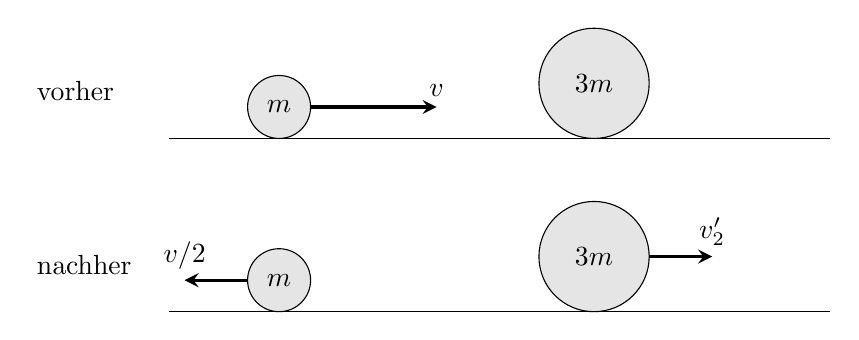
\begin{tikzpicture}[>=stealth]
 \node[anchor=west] at (0,0.6) {vorher};
 \draw (1.8,0) -- (10.2,0);
 \draw[fill=gray!20] (3.2,0.4) circle (0.4);
 \node at (3.2,0.4) {$m$};
 \draw[->, very thick] (3.6,0.4) -- (5.2,0.4) node[above] {$v$};
 \draw[fill=gray!20] (7.2,0.7) circle (0.7);
 \node at (7.2,0.7) {$3m$};
 \node[anchor=west] at (0,-1.6) {nachher};
 \draw (1.8,-2.2) -- (10.2,-2.2);
 \draw[fill=gray!20] (3.2,-1.8) circle (0.4);
 \node at (3.2,-1.8) {$m$};
 \draw[->, very thick] (2.8,-1.8) -- (2,-1.8) node[above] {$v/2$};
 \draw[fill=gray!20] (7.2,-1.5) circle (0.7);
 \node at (7.2,-1.5) {$3m$};
 \draw[->, very thick] (7.9,-1.5) -- (8.7,-1.5) node[above] {$v_2'$};
\end{tikzpicture}
\end{center}

Die ursprüngliche Bewegungsrichtung der ersten Kugel ist positiv. Nach dem Stoss hat die erste Kugel die Geschwindigkeit $-v/2$. Impulserhaltung:
\begin{align}
 m\,v &= m\cdot\left(-\frac{v}{2}\right) + 3m\,v_2' \\
 3\,v_2' &= v + \frac{v}{2} = \frac{3}{2}\,v \\
 v_2' &= \result{\frac{v}{2}}
\end{align}
Die zweite Kugel bewegt sich mit halber Anfangsgeschwindigkeit in die ursprüngliche Richtung weiter.
